\documentclass[aspectratio=169]{beamer}
\usepackage[utf8]{inputenc}
\usepackage[T1]{fontenc}
\usepackage{booktabs}
\usepackage{colortbl}
\usepackage{graphicx}
\usepackage{xcolor}
\usepackage{tikz}
\usetikzlibrary{positioning}
\usepackage{pgfplots}
\pgfplotsset{compat=1.18}
\usepackage{amsmath}
\usepackage{tcolorbox}
\tcbuselibrary{skins}

\definecolor{cdark}{HTML}{0D2137}
\definecolor{cmid}{HTML}{065A82}
\definecolor{cteal}{HTML}{02C39A}
\definecolor{clight}{HTML}{E8F4F8}
\definecolor{ctext}{HTML}{1A2E40}
\definecolor{cmuted}{HTML}{607D8B}
\definecolor{cwarn}{HTML}{F4A261}
\definecolor{cgap}{HTML}{E63946}
\definecolor{caccent}{HTML}{A0BFD0}
\definecolor{cbg2}{HTML}{028090}

\usetheme{default}
\usecolortheme{default}
\setbeamertemplate{navigation symbols}{}
\usefonttheme{professionalfonts}
\setbeamerfont{frametitle}{size=\large,series=\bfseries}
\setbeamercolor{frametitle}{fg=cdark,bg=white}
\setbeamercolor{normal text}{fg=ctext}
\setbeamercolor{background canvas}{bg=white}
\setbeamercolor{item}{fg=cteal}

\addtobeamertemplate{frametitle}{}{%
  \vspace{-4pt}\textcolor{cteal}{\hrule height 1.5pt}\vspace{3pt}}

\setbeamertemplate{footline}{%
  \leavevmode\hbox{%
    \begin{beamercolorbox}[wd=0.85\paperwidth,ht=2.2ex,dp=1ex,leftskip=4pt]{normal text}%
      \tiny\color{cmuted}Project Team — xai-spatio-temporal
    \end{beamercolorbox}%
    \begin{beamercolorbox}[wd=0.15\paperwidth,ht=2.2ex,dp=1ex,right,rightskip=6pt]{normal text}%
      \scriptsize\color{cmuted}\insertframenumber/\inserttotalframenumber%
    \end{beamercolorbox}}}

\setbeamertemplate{itemize item}{\color{cteal}\textbullet}
\setbeamertemplate{itemize subitem}{\color{cmid}--}
\setlength{\leftmargini}{1em}

\newcommand{\statcard}[3]{%
  \begin{tcolorbox}[enhanced,boxrule=1pt,arc=2pt,
      colback=clight,colframe=cmid,
      top=3pt,bottom=3pt,left=3pt,right=3pt]
    \centering
    {\color{cmid}\large\bfseries\parbox[c][2.7em][c]{\linewidth}{\centering #1}}\\[1pt]
    {\color{ctext}\bfseries\tiny\parbox[c][2.8em][c]{\linewidth}{\centering #2}}\\[1pt]
    {\color{cmuted}\tiny\parbox[c][2.8em][c]{\linewidth}{\centering #3}}
  \end{tcolorbox}}

\title{Picoclimate — Shapelets EDA \& Clustering Summary}
\subtitle{Shapelet selection, clustering and alignment notes}
\author{Project Team}
\date{May 29, 2026}

\begin{document}

% Title
{\setbeamercolor{background canvas}{bg=cdark}
\begin{frame}[plain]
\begin{tikzpicture}[remember picture,overlay]
  \fill[cteal](current page.north west)rectangle([xshift=6pt]current page.south west);
\end{tikzpicture}
\vspace{1.1cm}
{\color{white}\huge\bfseries PICOPATT / Picoclimate}\\[5pt]
{\color{cteal}\large\itshape Shapelets EDA \& Clustering Summary --- May 29, 2026}\\[8pt]
{\color{caccent}\small Explainable Clustering for Spatio-Temporal Picoclimatic Data}\\[0.6cm]
{\color{cmid}\rule{5.2cm}{0.8pt}}\\[5pt]
{\color{caccent}\footnotesize\textbf{Project Team}}\\[2pt]
{\color{caccent}\footnotesize May 29, 2026}
\end{frame}}

% Run summary
\begin{frame}{Run summary}
\begin{itemize}
  \item Data: \texttt{data/picoclimate\_test/tracks\_measurements.csv} -> aggregated windows
  \item Rows (windows): 165; Slot-columns: 100
  \item Selected shapelets: 74; KMeans best k=2; KMeans silhouette=0.313
  \item Ward silhouette=0.313; HDBSCAN: unavailable in env
\end{itemize}
\end{frame}

% Data structure
\begin{frame}{Data structure and daily windows}
\begin{itemize}
  \item Raw fixture is track-based: each \texttt{track\_id} is an ordered sequence of measurements.
  \item If \texttt{loc\_id} follows the visit order, it can be treated as a pseudo-time slot axis for a track.
  \item For daily summaries, group by \texttt{track\_id + date + time\_slot} and keep a fixed slot order.
  \item If the raw order is irregular, align first, then resample to a common length before extracting shapelets.
\end{itemize}
\begin{block}{Practical rule}
Use the real time columns when available; use \texttt{loc\_id} ordering only as a fallback pseudo-time index.
\end{block}
\end{frame}

% Why window features
\begin{frame}{Why \texttt{window\_features.csv} still matters}
\begin{itemize}
  \item It is a fixed-width table built from the track fixture, so clustering and EDA are reproducible and cheap.
  \item It lets us compare shapelet-distance clustering against a simpler baseline on the same windows.
  \item It decouples two questions: representation quality and clustering quality.
  \item For today\textquotesingle s meeting, it is the stable input that feeds the current shapelet pipeline and slide figures.
\end{itemize}
\end{frame}

% Silhouette figure
\begin{frame}{Silhouette by method}
\begin{center}
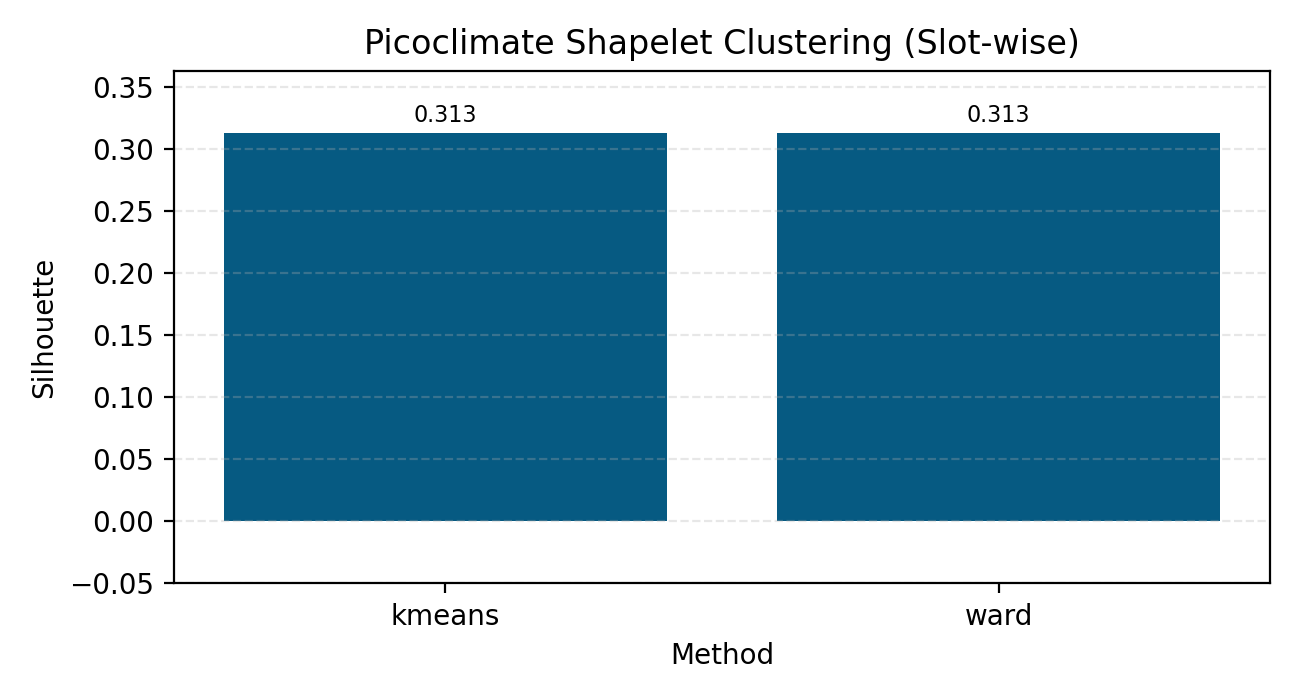
\includegraphics[width=0.85\textwidth]{../../../scripts/figures/picoclimate_shapelet_results_2026-05-29.png}
\end{center}
\end{frame}

% EDA: track length distribution
\begin{frame}{EDA — Track length distribution}
\begin{center}
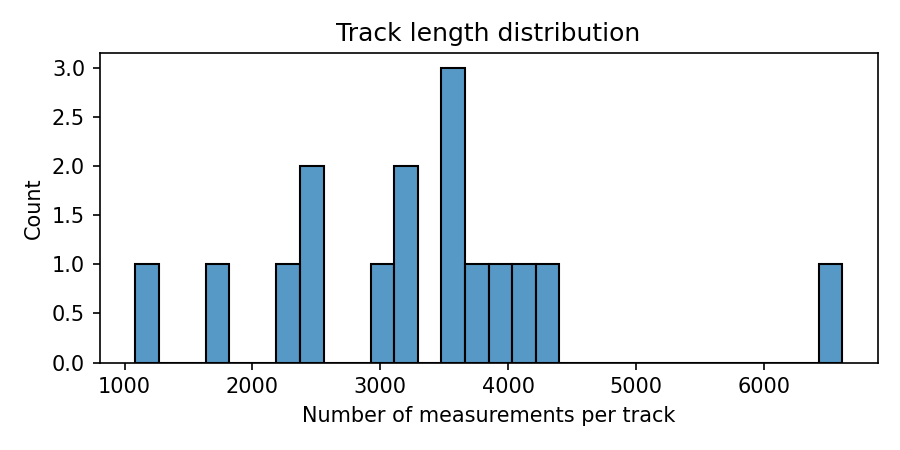
\includegraphics[width=0.85\textwidth]{../../../scripts/figures/picoclimate_track_length_dist.png}
\end{center}
\end{frame}

% EDA: numeric histograms
\begin{frame}{EDA — Numeric histograms (top variables)}
\begin{center}
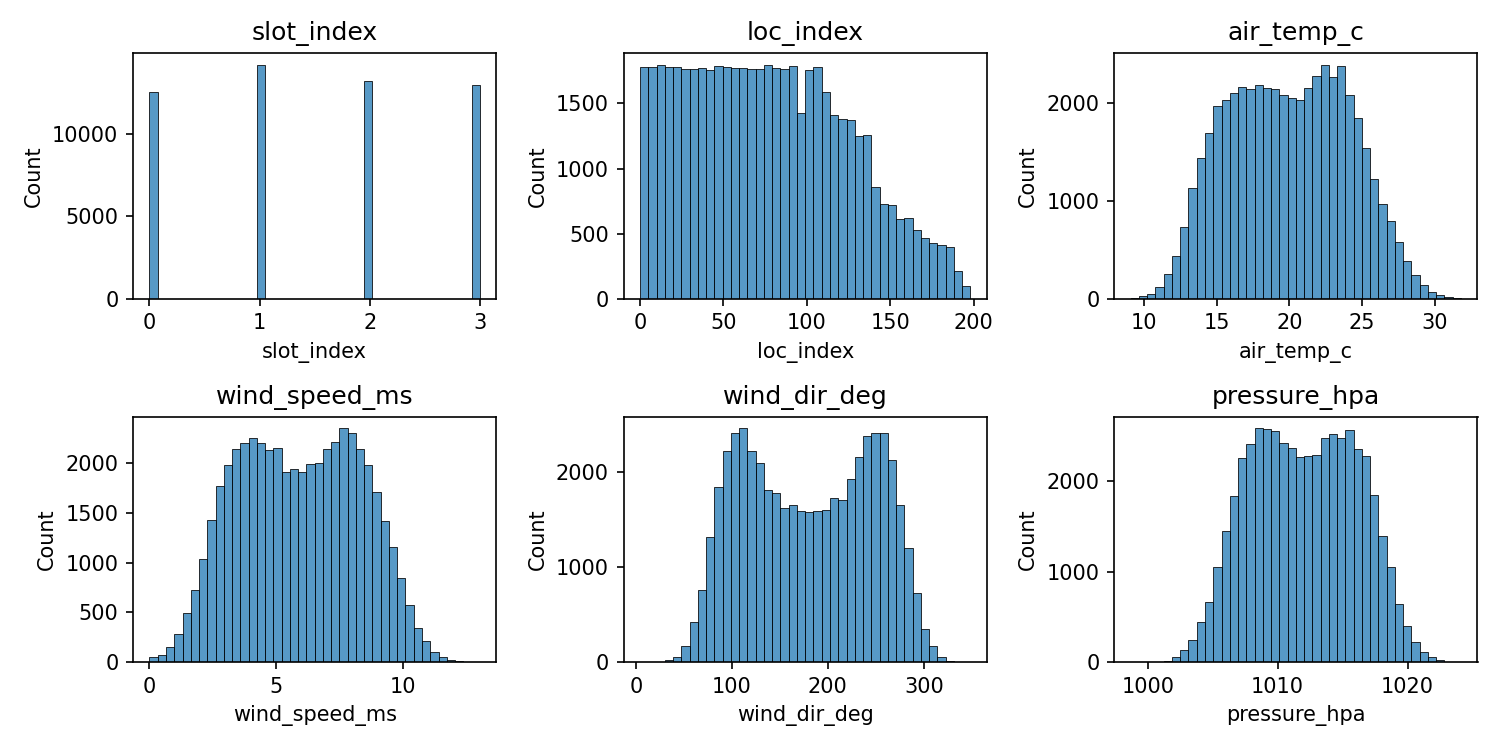
\includegraphics[width=0.9\textwidth]{../../../scripts/figures/picoclimate_numeric_hist_topvars.png}
\end{center}
\end{frame}

% EDA: sample time-series
\begin{frame}{EDA — Sample time-series}
\begin{center}
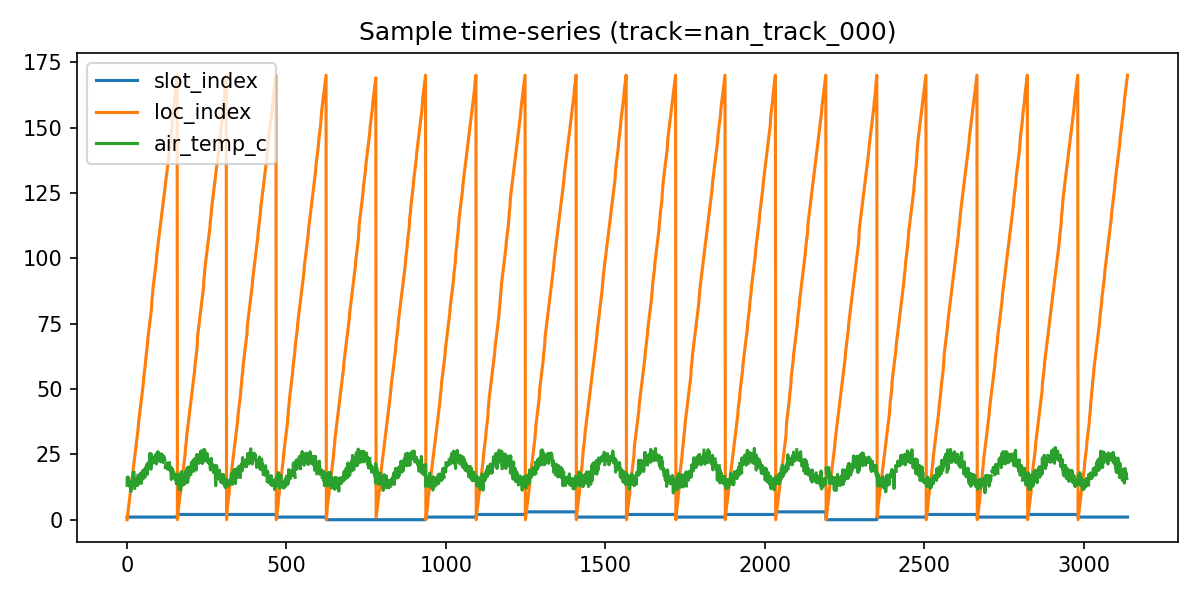
\includegraphics[width=0.9\textwidth]{../../../scripts/figures/picoclimate_sample_timeseries.png}
\end{center}
\end{frame}

% Statistics slide
\begin{frame}{Shapelet run statistics}
\begin{itemize}
  \item Selected shapelets: 74
  \item Candidate pool: 1000; rows (windows): 165; slot-columns: 100
\end{itemize}
\vspace{6pt}
\begin{block}{KMeans silhouette by k (selected)}
\begin{tabular}{lr}
\toprule
k & silhouette \\
\midrule
2 & 0.3133 \\
3 & 0.1493 \\
4 & 0.1586 \\
5 & 0.1374 \\
6 & 0.1280 \\
\bottomrule
\end{tabular}
\end{block}
\vspace{6pt}
\footnotesize Detailed outputs: docs/reports/picoclimate_2026-05-29/
\end{frame}

% Alignment slide
\begin{frame}{Alignment / Resampling (notes)}
\begin{block}{Key approach}
\begin{itemize}
  \item Endpoint extension + Catmull--Rom spline resampling to homogenize mixed-length segments.
  \item Smooth + resample each indicator to fixed length prior to shapelet scoring and clustering.
  \item Implementation: see \texttt{scripts/alignment.txt} for \texttt{rescale\_and\_smooth} and \texttt{rescale\_and\_smooth\_2d} helpers.
\end{itemize}
\end{block}
\vspace{6pt}
\begin{tcolorbox}[colback=clight,colframe=cmid]
\footnotesize Example functions: \texttt{extend\_points}, \texttt{rescale\_and\_smooth}, \texttt{rescale\_and\_smooth\_2d} (Catmull--Rom)
\end{tcolorbox}
\end{frame}

% Next steps
\begin{frame}{Next steps for meeting}
\begin{itemize}
  \item Present EDA figures: track-lengths, numeric histograms, sample time-series.
  \item Explain pipeline: tracks -> window\_features -> mixed-length shapelets -> shapelet-distance matrix -> KMeans -> surrogate explanations (SHAP and abductive edits).
  \item Discuss clustering strategies: by month/year, by location subset, or data-driven (subspace clustering); cover trade-offs.
  \item Immediate actions: add per-shapelet stats (mean/std/max), export cluster summaries CSV, and prepare brief report slides.
\end{itemize}
\end{frame}

\end{document}
